\documentclass{article}

\usepackage[utf8]{inputenc}
\usepackage[ngerman]{babel}
% Figures
\usepackage{graphicx}
\usepackage{float}

% Tables
\usepackage{makecell}
\usepackage{multirow}
\usepackage{rotating}
\usepackage{booktabs}

% BibTeX configuration
\usepackage{biblatex}
\bibliography{references} 
\RequirePackage{doi}
\usepackage{hyperref}
\usepackage{csquotes}
\usepackage{enumitem} 




\title{Assignment 1}
\author{Yannick Lang\\
    \small yannick-stephan.lang@stud.uni-bamberg.de}

\date{ \vspace{0.5cm} \large 
UxD-UIxD-M\\ 
  \emph{Urban Interaction Design} \\ \vspace{0.2cm}
  Otto-Friedrich-Universität Bamberg \\ \vspace{0.2cm}
  Wintersemester 2024/25}

\begin{document}

\maketitle

% Main contents
\section{Lokalisierung}

\subsection{Trilateration}
\subsection{GPS Koordinaten}
\label{sec:coord-conversion}

Um Koordinaten zwischen den verschiedenen Formaten zu konvertieren, habe ich eine kleine Webapp geschrieben.

Dazu habe ich folgende Annahmen getroffen:

\begin{itemize}[align=left, leftmargin=*]
    \item[\textbf{Google KML}] Hier handelt es sich um ein Dezimalgrad System, die Angaben werden als (lat, lon) gewertet (also wie (vermutlich) in der Angabe und nicht wie in den KML Dateien, die man bei GoogleMaps herunterladen kann). Die Wertebereiche sind (-90, 90) für lat und (-180, 180) für lon.
    \item[\textbf{NMEA 0132}] Mischung aus Grad und Dezimalminuten, also DDMM.MMM. führende Nullen werden gegebenenfalls nicht ausgegeben. Die Wertebereiche sind (0, 90) für lat und (0, 180) für lon, zusätzlich werden die Richtungen N, S, E, W angegeben.
    \item[\textbf{JPEG EXIF}] Hier handelt es sich um ein Grad, Minuten, Sekunden System, die Angaben werden als (lat, lon) gewertet. Die Wertebereiche sind (-90, 90) für lat-Grad (-180, 180) für lon-Grad und jeweils (0, 60) für Minuten und Sekunden. Sekunden können Nachkommastellen haben. Statt der Vorzeichen bei den Grad kann die Richtung N, S, E, W angegeben werden. Grad, Minuten und Sekunden sind durch die jeweiligen Einheitenzeichen (°,',") oder durch Strickpunkte (;) getrennt. Formate wie das auf Wikipedia verwendete (zu beachten: Richtungen nach statt vor den Koordinaten und zwar ähnliche aber andere Symbole für Minuten und Sekunden) werden aktuell nicht unterstützt.
\end{itemize}

Der Source Code ist auf GitHub\footnote{\url{https://github.com/layaxx/coordinate-conversion}} zu finden und auch anbei als Teil der Abgabe. Die WebApp kann durch Öffnen der Datei \verb|dist/index.html| in einem Browser gestartet werden und ist im Internet\footnote{\url{https://layaxx.github.io/coordinate-conversion}} verfügbar.

Es existiert ein Eingabefeld, in das Koordinaten in einem der oben beschriebenen Formate kopiert werden können. Die App erkennt das Format und berechnet automatisch die entsprechenden anderen Formate.

Außerdem gibt es für jeden Bestandteil von jedem Koordinatenformat ein extra Eingabefeld, mit dem man diesen Bestandteil anpassen kann. Alle anderen Formate werden automatisch angepasst.
\subsection{Distanz}

Die Distanzkalkulation zwischen zwei Punkten ist in der selben, oben beschriebenen, Webapp implementiert. Hierzu gibt es zwei Eingabefelder, in die Koordinaten in einem beliebigen der oben genannten Formate eingegeben oder einkopiert werden können. Die Koordinaten werden anschließend in Dezimalgrad umgerechnet. Mittel der Haversine Formel wird die Distanz zwischen den beiden Punkten ermittelt und ausgegeben.

Zusätzlich sind die Beispiele aus der Angabe mit der jeweiligen Distanz enthalten. Durch Klicken auf die Koordinaten können diese auch direkt in die interaktive Distanzermittlung übernommen werden. Außerdem ist natürlich ein Kopieren und Einfügen möglich.

\begin{figure}[h]
    \centering
    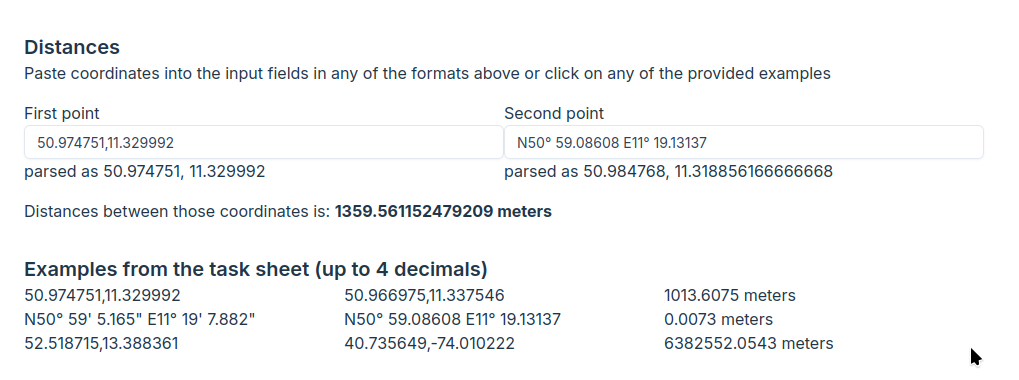
\includegraphics[width=0.9\textwidth]{figures/distanzkalkulation.png}
    \caption{Screenshot aus der WebApp. Zu sehen sind hier neben den Distanzen zu den Beispielen aus der Angabe auch die mögliche Mischung von Eingabeformaten.}
    \label{distanzkalkulation}
\end{figure}
\section{\enquote{In the Wild}}
\subsection{RSSI}
\subsection{WiFi Scanning (Wardriving)}
\subsection{Geo-Caching}

% Please clean your references! 
% See https://sites.umiacs.umd.edu/elm/2018/12/13/the-art-of-clean-references/
\printbibliography


\end{document}